\documentclass[twoside]{book}

% Packages required by doxygen
\usepackage{fixltx2e}
\usepackage{calc}
\usepackage{doxygen}
\usepackage[export]{adjustbox} % also loads graphicx
\usepackage{graphicx}
\usepackage[utf8]{inputenc}
\usepackage{makeidx}
\usepackage{multicol}
\usepackage{multirow}
\PassOptionsToPackage{warn}{textcomp}
\usepackage{textcomp}
\usepackage[nointegrals]{wasysym}
\usepackage[table]{xcolor}

% Font selection
\usepackage[T1]{fontenc}
\usepackage[scaled=.90]{helvet}
\usepackage{courier}
\usepackage{amssymb}
\usepackage{sectsty}
\renewcommand{\familydefault}{\sfdefault}
\allsectionsfont{%
  \fontseries{bc}\selectfont%
  \color{darkgray}%
}
\renewcommand{\DoxyLabelFont}{%
  \fontseries{bc}\selectfont%
  \color{darkgray}%
}
\newcommand{\+}{\discretionary{\mbox{\scriptsize$\hookleftarrow$}}{}{}}

% Page & text layout
\usepackage{geometry}
\geometry{%
  a4paper,%
  top=2.5cm,%
  bottom=2.5cm,%
  left=2.5cm,%
  right=2.5cm%
}
\tolerance=750
\hfuzz=15pt
\hbadness=750
\setlength{\emergencystretch}{15pt}
\setlength{\parindent}{0cm}
\setlength{\parskip}{3ex plus 2ex minus 2ex}
\makeatletter
\renewcommand{\paragraph}{%
  \@startsection{paragraph}{4}{0ex}{-1.0ex}{1.0ex}{%
    \normalfont\normalsize\bfseries\SS@parafont%
  }%
}
\renewcommand{\subparagraph}{%
  \@startsection{subparagraph}{5}{0ex}{-1.0ex}{1.0ex}{%
    \normalfont\normalsize\bfseries\SS@subparafont%
  }%
}
\makeatother

% Headers & footers
\usepackage{fancyhdr}
\pagestyle{fancyplain}
\fancyhead[LE]{\fancyplain{}{\bfseries\thepage}}
\fancyhead[CE]{\fancyplain{}{}}
\fancyhead[RE]{\fancyplain{}{\bfseries\leftmark}}
\fancyhead[LO]{\fancyplain{}{\bfseries\rightmark}}
\fancyhead[CO]{\fancyplain{}{}}
\fancyhead[RO]{\fancyplain{}{\bfseries\thepage}}
\fancyfoot[LE]{\fancyplain{}{}}
\fancyfoot[CE]{\fancyplain{}{}}
\fancyfoot[RE]{\fancyplain{}{\bfseries\scriptsize Generated by Doxygen }}
\fancyfoot[LO]{\fancyplain{}{\bfseries\scriptsize Generated by Doxygen }}
\fancyfoot[CO]{\fancyplain{}{}}
\fancyfoot[RO]{\fancyplain{}{}}
\renewcommand{\footrulewidth}{0.4pt}
\renewcommand{\chaptermark}[1]{%
  \markboth{#1}{}%
}
\renewcommand{\sectionmark}[1]{%
  \markright{\thesection\ #1}%
}

% Indices & bibliography
\usepackage{natbib}
\usepackage[titles]{tocloft}
\setcounter{tocdepth}{3}
\setcounter{secnumdepth}{5}
\makeindex

% Hyperlinks (required, but should be loaded last)
\usepackage{ifpdf}
\ifpdf
  \usepackage[pdftex,pagebackref=true]{hyperref}
\else
  \usepackage[ps2pdf,pagebackref=true]{hyperref}
\fi
\hypersetup{%
  colorlinks=true,%
  linkcolor=blue,%
  citecolor=blue,%
  unicode%
}

% Custom commands
\newcommand{\clearemptydoublepage}{%
  \newpage{\pagestyle{empty}\cleardoublepage}%
}

\usepackage{caption}
\captionsetup{labelsep=space,justification=centering,font={bf},singlelinecheck=off,skip=4pt,position=top}

%===== C O N T E N T S =====

\begin{document}

% Titlepage & ToC
\hypersetup{pageanchor=false,
             bookmarksnumbered=true,
             pdfencoding=unicode
            }
\pagenumbering{alph}
\begin{titlepage}
\vspace*{7cm}
\begin{center}%
{\Large Hashcount }\\
\vspace*{1cm}
{\large Generated by Doxygen 1.8.13}\\
\end{center}
\end{titlepage}
\clearemptydoublepage
\pagenumbering{roman}
\tableofcontents
\clearemptydoublepage
\pagenumbering{arabic}
\hypersetup{pageanchor=true}

%--- Begin generated contents ---
\chapter{Class Index}
\section{Class List}
Here are the classes, structs, unions and interfaces with brief descriptions\+:\begin{DoxyCompactList}
\item\contentsline{section}{\hyperlink{structhashlist}{hashlist} \\*A dynamic list of hash buckets }{\pageref{structhashlist}}{}
\item\contentsline{section}{\hyperlink{structwordlist}{wordlist} \\*Is a header that provides multible Functions for hashlists and wordlists. Author\+: Parzer Florian }{\pageref{structwordlist}}{}
\end{DoxyCompactList}

\chapter{File Index}
\section{File List}
Here is a list of all files with brief descriptions\+:\begin{DoxyCompactList}
\item\contentsline{section}{src/\hyperlink{Hashcount_8c}{Hashcount.\+c} }{\pageref{Hashcount_8c}}{}
\item\contentsline{section}{src/\hyperlink{hashcount__func_8c}{hashcount\+\_\+func.\+c} }{\pageref{hashcount__func_8c}}{}
\item\contentsline{section}{src/\hyperlink{hashcount__func_8h}{hashcount\+\_\+func.\+h} }{\pageref{hashcount__func_8h}}{}
\end{DoxyCompactList}

\chapter{Class Documentation}
\hypertarget{structhashlist}{}\section{hashlist Struct Reference}
\label{structhashlist}\index{hashlist@{hashlist}}


A dynamic list of hash buckets.  




{\ttfamily \#include $<$hashcount\+\_\+func.\+h$>$}



Collaboration diagram for hashlist\+:\nopagebreak
\begin{figure}[H]
\begin{center}
\leavevmode
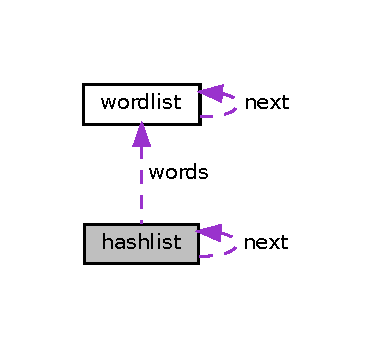
\includegraphics[width=179pt]{structhashlist__coll__graph}
\end{center}
\end{figure}
\subsection*{Public Attributes}
\begin{DoxyCompactItemize}
\item 
struct \hyperlink{structhashlist}{hashlist} $\ast$ \hyperlink{structhashlist_ac31c298110f5630adfb6e051cf8657ac}{next}
\item 
\hyperlink{structwordlist}{wordlist} $\ast$ \hyperlink{structhashlist_a62f143e3e8911dccb242579a7f06e973}{words}
\item 
int \hyperlink{structhashlist_aab67bf6a16fd9f0ae1ad7190acc95298}{hash}
\end{DoxyCompactItemize}


\subsection{Detailed Description}
A dynamic list of hash buckets. 

It is a dynamic list where each element has a pointer to the next element, a pointer to a wordlist and the hash value 

\subsection{Member Data Documentation}
\mbox{\Hypertarget{structhashlist_aab67bf6a16fd9f0ae1ad7190acc95298}\label{structhashlist_aab67bf6a16fd9f0ae1ad7190acc95298}} 
\index{hashlist@{hashlist}!hash@{hash}}
\index{hash@{hash}!hashlist@{hashlist}}
\subsubsection{\texorpdfstring{hash}{hash}}
{\footnotesize\ttfamily int hashlist\+::hash}

The list of words with the same hash value \mbox{\Hypertarget{structhashlist_ac31c298110f5630adfb6e051cf8657ac}\label{structhashlist_ac31c298110f5630adfb6e051cf8657ac}} 
\index{hashlist@{hashlist}!next@{next}}
\index{next@{next}!hashlist@{hashlist}}
\subsubsection{\texorpdfstring{next}{next}}
{\footnotesize\ttfamily struct \hyperlink{structhashlist}{hashlist}$\ast$ hashlist\+::next}

\mbox{\Hypertarget{structhashlist_a62f143e3e8911dccb242579a7f06e973}\label{structhashlist_a62f143e3e8911dccb242579a7f06e973}} 
\index{hashlist@{hashlist}!words@{words}}
\index{words@{words}!hashlist@{hashlist}}
\subsubsection{\texorpdfstring{words}{words}}
{\footnotesize\ttfamily \hyperlink{structwordlist}{wordlist}$\ast$ hashlist\+::words}

The next bucket of the lsit 

The documentation for this struct was generated from the following file\+:\begin{DoxyCompactItemize}
\item 
src/\hyperlink{hashcount__func_8h}{hashcount\+\_\+func.\+h}\end{DoxyCompactItemize}

\hypertarget{structwordlist}{}\section{wordlist Struct Reference}
\label{structwordlist}\index{wordlist@{wordlist}}


Is a header that provides multible Functions for hashlists and wordlists. Author\+: Parzer Florian.  




{\ttfamily \#include $<$hashcount\+\_\+func.\+h$>$}



Collaboration diagram for wordlist\+:\nopagebreak
\begin{figure}[H]
\begin{center}
\leavevmode
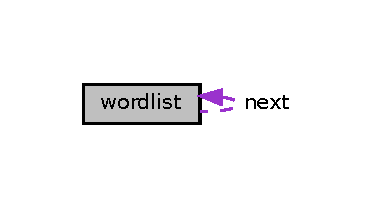
\includegraphics[width=179pt]{structwordlist__coll__graph}
\end{center}
\end{figure}
\subsection*{Public Attributes}
\begin{DoxyCompactItemize}
\item 
struct \hyperlink{structwordlist}{wordlist} $\ast$ \hyperlink{structwordlist_a6a9fb0cf06d47f1bf57f0c71889cb889}{next}
\item 
int \hyperlink{structwordlist_a472cb03a36de8c3507bcf07abf56a607}{count}
\item 
char $\ast$ \hyperlink{structwordlist_adf182e526a01f9bcf7e01e869a7de1a3}{word}
\end{DoxyCompactItemize}


\subsection{Detailed Description}
Is a header that provides multible Functions for hashlists and wordlists. Author\+: Parzer Florian. 

A dynamic list of words

It is a dynamic list where eac element has a pointer to the next element, an integer variable that is used for counting and the word itself 

\subsection{Member Data Documentation}
\mbox{\Hypertarget{structwordlist_a472cb03a36de8c3507bcf07abf56a607}\label{structwordlist_a472cb03a36de8c3507bcf07abf56a607}} 
\index{wordlist@{wordlist}!count@{count}}
\index{count@{count}!wordlist@{wordlist}}
\subsubsection{\texorpdfstring{count}{count}}
{\footnotesize\ttfamily int wordlist\+::count}

The next element of the lsit \mbox{\Hypertarget{structwordlist_a6a9fb0cf06d47f1bf57f0c71889cb889}\label{structwordlist_a6a9fb0cf06d47f1bf57f0c71889cb889}} 
\index{wordlist@{wordlist}!next@{next}}
\index{next@{next}!wordlist@{wordlist}}
\subsubsection{\texorpdfstring{next}{next}}
{\footnotesize\ttfamily struct \hyperlink{structwordlist}{wordlist}$\ast$ wordlist\+::next}

\mbox{\Hypertarget{structwordlist_adf182e526a01f9bcf7e01e869a7de1a3}\label{structwordlist_adf182e526a01f9bcf7e01e869a7de1a3}} 
\index{wordlist@{wordlist}!word@{word}}
\index{word@{word}!wordlist@{wordlist}}
\subsubsection{\texorpdfstring{word}{word}}
{\footnotesize\ttfamily char$\ast$ wordlist\+::word}

The number of times the word was found 

The documentation for this struct was generated from the following file\+:\begin{DoxyCompactItemize}
\item 
src/\hyperlink{hashcount__func_8h}{hashcount\+\_\+func.\+h}\end{DoxyCompactItemize}

\chapter{File Documentation}
\hypertarget{Hashcount_8c}{}\section{src/\+Hashcount.c File Reference}
\label{Hashcount_8c}\index{src/\+Hashcount.\+c@{src/\+Hashcount.\+c}}
{\ttfamily \#include $<$getopt.\+h$>$}\newline
{\ttfamily \#include $<$stdio.\+h$>$}\newline
{\ttfamily \#include $<$stdlib.\+h$>$}\newline
{\ttfamily \#include $<$string.\+h$>$}\newline
{\ttfamily \#include \char`\"{}hashcount\+\_\+func.\+h\char`\"{}}\newline
{\ttfamily \#include $<$unistd.\+h$>$}\newline
Include dependency graph for Hashcount.\+c\+:\nopagebreak
\begin{figure}[H]
\begin{center}
\leavevmode
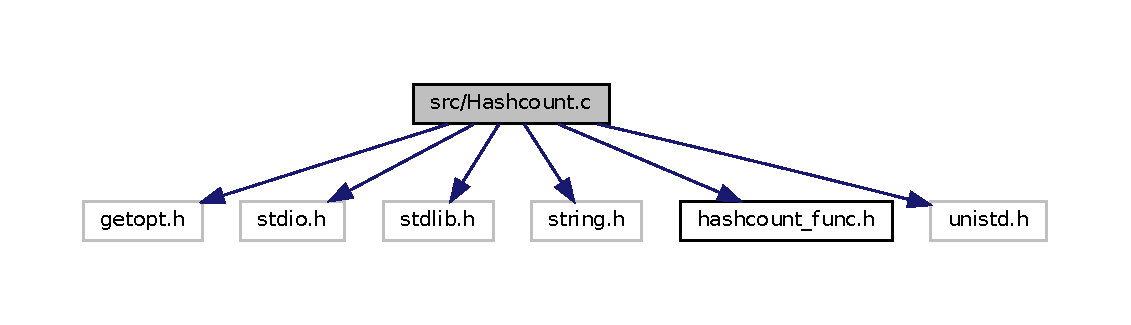
\includegraphics[width=350pt]{Hashcount_8c__incl}
\end{center}
\end{figure}
\subsection*{Functions}
\begin{DoxyCompactItemize}
\item 
int \hyperlink{Hashcount_8c_a0ddf1224851353fc92bfbff6f499fa97}{main} (int argc, char $\ast$argv\mbox{[}$\,$\mbox{]})
\begin{DoxyCompactList}\small\item\em Is a header that provides multible Functions for hashlists and wordlists. Author\+: Parzer Florian. \end{DoxyCompactList}\end{DoxyCompactItemize}


\subsection{Function Documentation}
\mbox{\Hypertarget{Hashcount_8c_a0ddf1224851353fc92bfbff6f499fa97}\label{Hashcount_8c_a0ddf1224851353fc92bfbff6f499fa97}} 
\index{Hashcount.\+c@{Hashcount.\+c}!main@{main}}
\index{main@{main}!Hashcount.\+c@{Hashcount.\+c}}
\subsubsection{\texorpdfstring{main()}{main()}}
{\footnotesize\ttfamily int main (\begin{DoxyParamCaption}\item[{int}]{argc,  }\item[{char $\ast$}]{argv\mbox{[}$\,$\mbox{]} }\end{DoxyParamCaption})}



Is a header that provides multible Functions for hashlists and wordlists. Author\+: Parzer Florian. 

The main methode of the programm

This methode handles the user input and starts depending on it various other methodes


\begin{DoxyParams}{Parameters}
{\em argc} & The number of arguments that the user has written \\
\hline
{\em argv} & The arguments that the user has written \\
\hline
\end{DoxyParams}
\begin{DoxyReturn}{Returns}
if there were no errors\+: 0. Otherwhise -\/1 
\end{DoxyReturn}

\hypertarget{hashcount__func_8c}{}\section{src/hashcount\+\_\+func.c File Reference}
\label{hashcount__func_8c}\index{src/hashcount\+\_\+func.\+c@{src/hashcount\+\_\+func.\+c}}
{\ttfamily \#include $<$stdio.\+h$>$}\newline
{\ttfamily \#include $<$stdlib.\+h$>$}\newline
{\ttfamily \#include $<$string.\+h$>$}\newline
{\ttfamily \#include $<$ctype.\+h$>$}\newline
{\ttfamily \#include \char`\"{}hashcount\+\_\+func.\+h\char`\"{}}\newline
Include dependency graph for hashcount\+\_\+func.\+c\+:\nopagebreak
\begin{figure}[H]
\begin{center}
\leavevmode
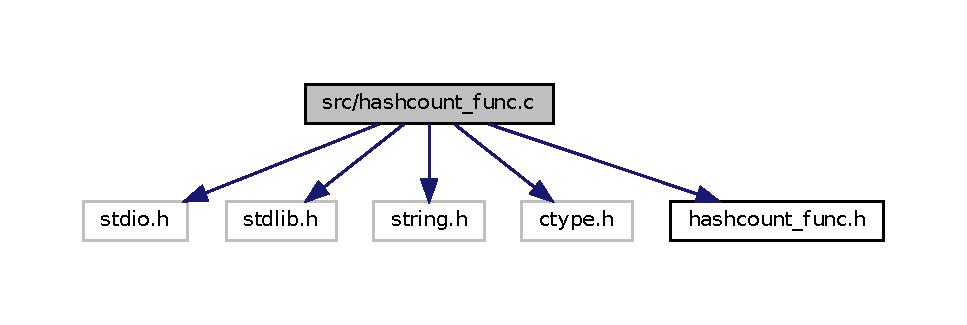
\includegraphics[width=350pt]{hashcount__func_8c__incl}
\end{center}
\end{figure}
\subsection*{Functions}
\begin{DoxyCompactItemize}
\item 
void \hyperlink{hashcount__func_8c_a13ed1a138272530c9f87f3071016c374}{add\+Word\+To\+Bucket} (\hyperlink{structhashlist}{hashlist} $\ast$$\ast$list, int hash, char $\ast$word)
\begin{DoxyCompactList}\small\item\em Provides multible Functions for hashlists and wordlists. Author\+: Parzer Florian. \end{DoxyCompactList}\item 
void \hyperlink{hashcount__func_8c_ad1b217640d5373185b0ab4611b271a86}{read\+File} (\hyperlink{structhashlist}{hashlist} $\ast$$\ast$list, F\+I\+LE $\ast$file)
\begin{DoxyCompactList}\small\item\em Reads the File and fills the hashlist with the words of the file. \end{DoxyCompactList}\item 
int \hyperlink{hashcount__func_8c_aaa2b50e893200dda96cef15addbca050}{string\+Compare\+Lower} (char $\ast$word, char $\ast$other)
\begin{DoxyCompactList}\small\item\em Compares the lower case of two words. \end{DoxyCompactList}\item 
void \hyperlink{hashcount__func_8c_af5ab016cf90d6b793db2d24ab7fe6c0e}{add\+Word} (\hyperlink{structwordlist}{wordlist} $\ast$$\ast$list, char $\ast$word)
\begin{DoxyCompactList}\small\item\em Adds a word to the wordlist. \end{DoxyCompactList}\item 
void \hyperlink{hashcount__func_8c_af406ea8dc323ec35fd3512b182f08999}{free\+Hashlist} (\hyperlink{structhashlist}{hashlist} $\ast$list)
\begin{DoxyCompactList}\small\item\em Frees the with malloc allocated memory of a hashlist. \end{DoxyCompactList}\item 
int \hyperlink{hashcount__func_8c_a02e6d7eb6a614e0f0a00a7cf82805774}{get\+Hash} (char $\ast$word)
\begin{DoxyCompactList}\small\item\em Calculates the hashvalue of a word. \end{DoxyCompactList}\item 
void \hyperlink{hashcount__func_8c_a7ebd0e2c75c007cfa2a268bfce63c5e5}{print\+Hashlist} (\hyperlink{structhashlist}{hashlist} $\ast$list)
\begin{DoxyCompactList}\small\item\em Prints the hashlist in a readable way. \end{DoxyCompactList}\item 
void \hyperlink{hashcount__func_8c_afb73f9700e2348d754dabfbb3f85cd15}{print\+Hash\+Bucket} (\hyperlink{structhashlist}{hashlist} $\ast$list, long bucket)
\begin{DoxyCompactList}\small\item\em Prints on bucket of the hashlist. \end{DoxyCompactList}\item 
void \hyperlink{hashcount__func_8c_a79a2f0a71b4c8bd1716f9cb8d498d766}{print\+Buckets\+Words} (\hyperlink{structwordlist}{wordlist} $\ast$buckets, F\+I\+LE $\ast$file, F\+I\+LE $\ast$output)
\begin{DoxyCompactList}\small\item\em Only the words who have the same hash value as the stated buckets. \end{DoxyCompactList}\item 
void \hyperlink{hashcount__func_8c_a05d5a48c4befa15d197f866d8f8836a5}{print\+Censor\+Buckets} (\hyperlink{structwordlist}{wordlist} $\ast$buckets, F\+I\+LE $\ast$file, F\+I\+LE $\ast$output)
\begin{DoxyCompactList}\small\item\em Prints the text of the input file in the output file and censors the words in the stated buckets. \end{DoxyCompactList}\item 
int \hyperlink{hashcount__func_8c_a5c90d8b28888d7a264af0648ebf57b48}{contains} (char $\ast$word, \hyperlink{structwordlist}{wordlist} $\ast$buckets)
\begin{DoxyCompactList}\small\item\em Checks if the word has the same hash value as one of the buckets. \end{DoxyCompactList}\end{DoxyCompactItemize}


\subsection{Function Documentation}
\mbox{\Hypertarget{hashcount__func_8c_af5ab016cf90d6b793db2d24ab7fe6c0e}\label{hashcount__func_8c_af5ab016cf90d6b793db2d24ab7fe6c0e}} 
\index{hashcount\+\_\+func.\+c@{hashcount\+\_\+func.\+c}!add\+Word@{add\+Word}}
\index{add\+Word@{add\+Word}!hashcount\+\_\+func.\+c@{hashcount\+\_\+func.\+c}}
\subsubsection{\texorpdfstring{add\+Word()}{addWord()}}
{\footnotesize\ttfamily void add\+Word (\begin{DoxyParamCaption}\item[{\hyperlink{structwordlist}{wordlist} $\ast$$\ast$}]{list,  }\item[{char $\ast$}]{word }\end{DoxyParamCaption})}



Adds a word to the wordlist. 

Adds the word to the wordlist. If the word is already contained a counter is increased.


\begin{DoxyParams}{Parameters}
{\em list} & Is the wordlist in which the word is added. If it is N\+U\+LL, the list will be created. \\
\hline
{\em word} & The word the hash is calculated from. \\
\hline
\end{DoxyParams}
\mbox{\Hypertarget{hashcount__func_8c_a13ed1a138272530c9f87f3071016c374}\label{hashcount__func_8c_a13ed1a138272530c9f87f3071016c374}} 
\index{hashcount\+\_\+func.\+c@{hashcount\+\_\+func.\+c}!add\+Word\+To\+Bucket@{add\+Word\+To\+Bucket}}
\index{add\+Word\+To\+Bucket@{add\+Word\+To\+Bucket}!hashcount\+\_\+func.\+c@{hashcount\+\_\+func.\+c}}
\subsubsection{\texorpdfstring{add\+Word\+To\+Bucket()}{addWordToBucket()}}
{\footnotesize\ttfamily void add\+Word\+To\+Bucket (\begin{DoxyParamCaption}\item[{\hyperlink{structhashlist}{hashlist} $\ast$$\ast$}]{list,  }\item[{int}]{hash,  }\item[{char $\ast$}]{word }\end{DoxyParamCaption})}



Provides multible Functions for hashlists and wordlists. Author\+: Parzer Florian. 

Adds a word to a hashlist

Adds a word to the bucket of the hashlist with the hash of the parameter hash and adding the word to the wordlist in the bucket. If a element with the same hash does not exist, it will be created.


\begin{DoxyParams}{Parameters}
{\em list} & The hashlist to which the word is added. \\
\hline
{\em hash} & The hashvalue of the bucket to which the word will be added \\
\hline
{\em word} & The word the hash is calculated from \\
\hline
\end{DoxyParams}
\mbox{\Hypertarget{hashcount__func_8c_a5c90d8b28888d7a264af0648ebf57b48}\label{hashcount__func_8c_a5c90d8b28888d7a264af0648ebf57b48}} 
\index{hashcount\+\_\+func.\+c@{hashcount\+\_\+func.\+c}!contains@{contains}}
\index{contains@{contains}!hashcount\+\_\+func.\+c@{hashcount\+\_\+func.\+c}}
\subsubsection{\texorpdfstring{contains()}{contains()}}
{\footnotesize\ttfamily int contains (\begin{DoxyParamCaption}\item[{char $\ast$}]{word,  }\item[{\hyperlink{structwordlist}{wordlist} $\ast$}]{buckets }\end{DoxyParamCaption})}



Checks if the word has the same hash value as one of the buckets. 

Checks if the word has the same hash value as one of the buckets by comparing it to every element of the wordlist.


\begin{DoxyParams}{Parameters}
{\em word} & Is the word that is checked \\
\hline
{\em buckets} & Are the hash values that are compaired against \\
\hline
\end{DoxyParams}
\begin{DoxyReturn}{Returns}
1 if the word has the same hashv alue as one of the buckets, otherwise it will return 0 
\end{DoxyReturn}
\mbox{\Hypertarget{hashcount__func_8c_af406ea8dc323ec35fd3512b182f08999}\label{hashcount__func_8c_af406ea8dc323ec35fd3512b182f08999}} 
\index{hashcount\+\_\+func.\+c@{hashcount\+\_\+func.\+c}!free\+Hashlist@{free\+Hashlist}}
\index{free\+Hashlist@{free\+Hashlist}!hashcount\+\_\+func.\+c@{hashcount\+\_\+func.\+c}}
\subsubsection{\texorpdfstring{free\+Hashlist()}{freeHashlist()}}
{\footnotesize\ttfamily void free\+Hashlist (\begin{DoxyParamCaption}\item[{\hyperlink{structhashlist}{hashlist} $\ast$}]{list }\end{DoxyParamCaption})}



Frees the with malloc allocated memory of a hashlist. 

It iterates over every element of the hashlist and frees every element that reserved its memory with the melloc method


\begin{DoxyParams}{Parameters}
{\em list} & The hashlist that schould be freed \\
\hline
\end{DoxyParams}
\mbox{\Hypertarget{hashcount__func_8c_a02e6d7eb6a614e0f0a00a7cf82805774}\label{hashcount__func_8c_a02e6d7eb6a614e0f0a00a7cf82805774}} 
\index{hashcount\+\_\+func.\+c@{hashcount\+\_\+func.\+c}!get\+Hash@{get\+Hash}}
\index{get\+Hash@{get\+Hash}!hashcount\+\_\+func.\+c@{hashcount\+\_\+func.\+c}}
\subsubsection{\texorpdfstring{get\+Hash()}{getHash()}}
{\footnotesize\ttfamily int get\+Hash (\begin{DoxyParamCaption}\item[{char $\ast$}]{word }\end{DoxyParamCaption})}



Calculates the hashvalue of a word. 

Calculates the bash of the word by summing the values of the characters and calculate the result withc modulo


\begin{DoxyParams}{Parameters}
{\em word} & The word the hash is calculated from\\
\hline
\end{DoxyParams}
\begin{DoxyReturn}{Returns}
returns the calculated hashvalue as Integer 
\end{DoxyReturn}
\mbox{\Hypertarget{hashcount__func_8c_a79a2f0a71b4c8bd1716f9cb8d498d766}\label{hashcount__func_8c_a79a2f0a71b4c8bd1716f9cb8d498d766}} 
\index{hashcount\+\_\+func.\+c@{hashcount\+\_\+func.\+c}!print\+Buckets\+Words@{print\+Buckets\+Words}}
\index{print\+Buckets\+Words@{print\+Buckets\+Words}!hashcount\+\_\+func.\+c@{hashcount\+\_\+func.\+c}}
\subsubsection{\texorpdfstring{print\+Buckets\+Words()}{printBucketsWords()}}
{\footnotesize\ttfamily void print\+Buckets\+Words (\begin{DoxyParamCaption}\item[{\hyperlink{structwordlist}{wordlist} $\ast$}]{buckets,  }\item[{F\+I\+LE $\ast$}]{file,  }\item[{F\+I\+LE $\ast$}]{output }\end{DoxyParamCaption})}



Only the words who have the same hash value as the stated buckets. 

It prints only the words that\textquotesingle{}s hash maches one of the buckets. Every other character of the input file will not be printed.


\begin{DoxyParams}{Parameters}
{\em buckets} & The hash values of the stated buckets \\
\hline
{\em file} & The input file stream \\
\hline
{\em output} & The output file stream \\
\hline
\end{DoxyParams}
\mbox{\Hypertarget{hashcount__func_8c_a05d5a48c4befa15d197f866d8f8836a5}\label{hashcount__func_8c_a05d5a48c4befa15d197f866d8f8836a5}} 
\index{hashcount\+\_\+func.\+c@{hashcount\+\_\+func.\+c}!print\+Censor\+Buckets@{print\+Censor\+Buckets}}
\index{print\+Censor\+Buckets@{print\+Censor\+Buckets}!hashcount\+\_\+func.\+c@{hashcount\+\_\+func.\+c}}
\subsubsection{\texorpdfstring{print\+Censor\+Buckets()}{printCensorBuckets()}}
{\footnotesize\ttfamily void print\+Censor\+Buckets (\begin{DoxyParamCaption}\item[{\hyperlink{structwordlist}{wordlist} $\ast$}]{buckets,  }\item[{F\+I\+LE $\ast$}]{file,  }\item[{F\+I\+LE $\ast$}]{output }\end{DoxyParamCaption})}



Prints the text of the input file in the output file and censors the words in the stated buckets. 

It prints every character of the input file in the output file. If the word is contained in the stated buckets it will be censored.


\begin{DoxyParams}{Parameters}
{\em buckets} & The hash values of the stated buckets \\
\hline
{\em file} & The input file stream \\
\hline
{\em output} & The output file stream \\
\hline
\end{DoxyParams}
\mbox{\Hypertarget{hashcount__func_8c_afb73f9700e2348d754dabfbb3f85cd15}\label{hashcount__func_8c_afb73f9700e2348d754dabfbb3f85cd15}} 
\index{hashcount\+\_\+func.\+c@{hashcount\+\_\+func.\+c}!print\+Hash\+Bucket@{print\+Hash\+Bucket}}
\index{print\+Hash\+Bucket@{print\+Hash\+Bucket}!hashcount\+\_\+func.\+c@{hashcount\+\_\+func.\+c}}
\subsubsection{\texorpdfstring{print\+Hash\+Bucket()}{printHashBucket()}}
{\footnotesize\ttfamily void print\+Hash\+Bucket (\begin{DoxyParamCaption}\item[{\hyperlink{structhashlist}{hashlist} $\ast$}]{list,  }\item[{long}]{bucket }\end{DoxyParamCaption})}



Prints on bucket of the hashlist. 

Prints the stated bucket. If the words per line exeed 10 a new line is started. If the Bucket is not found it will print an error Message.


\begin{DoxyParams}{Parameters}
{\em list} & The hashlist in which the bucket will be searched in. \\
\hline
{\em bucket} & The hashvalue of the bucket that should be printed. \\
\hline
\end{DoxyParams}
\mbox{\Hypertarget{hashcount__func_8c_a7ebd0e2c75c007cfa2a268bfce63c5e5}\label{hashcount__func_8c_a7ebd0e2c75c007cfa2a268bfce63c5e5}} 
\index{hashcount\+\_\+func.\+c@{hashcount\+\_\+func.\+c}!print\+Hashlist@{print\+Hashlist}}
\index{print\+Hashlist@{print\+Hashlist}!hashcount\+\_\+func.\+c@{hashcount\+\_\+func.\+c}}
\subsubsection{\texorpdfstring{print\+Hashlist()}{printHashlist()}}
{\footnotesize\ttfamily void print\+Hashlist (\begin{DoxyParamCaption}\item[{\hyperlink{structhashlist}{hashlist} $\ast$}]{list }\end{DoxyParamCaption})}



Prints the hashlist in a readable way. 

Prints every bucket of the Hashlist in a seperate line. If the words per line exeed 10 a new line is started


\begin{DoxyParams}{Parameters}
{\em list} & The hashlist that will be printed. \\
\hline
\end{DoxyParams}
\mbox{\Hypertarget{hashcount__func_8c_ad1b217640d5373185b0ab4611b271a86}\label{hashcount__func_8c_ad1b217640d5373185b0ab4611b271a86}} 
\index{hashcount\+\_\+func.\+c@{hashcount\+\_\+func.\+c}!read\+File@{read\+File}}
\index{read\+File@{read\+File}!hashcount\+\_\+func.\+c@{hashcount\+\_\+func.\+c}}
\subsubsection{\texorpdfstring{read\+File()}{readFile()}}
{\footnotesize\ttfamily void read\+File (\begin{DoxyParamCaption}\item[{\hyperlink{structhashlist}{hashlist} $\ast$$\ast$}]{list,  }\item[{F\+I\+LE $\ast$}]{file }\end{DoxyParamCaption})}



Reads the File and fills the hashlist with the words of the file. 

The method reads the file. It splits the stream at the charackters \textquotesingle{}newline\textquotesingle{}, \textquotesingle{}space\textquotesingle{}, \textquotesingle{}.\textquotesingle{}, \textquotesingle{}\+:\textquotesingle{}, \textquotesingle{},\textquotesingle{}, \textquotesingle{};\textquotesingle{}, \textquotesingle{}?\textquotesingle{} and \textquotesingle{}space\textquotesingle{}. Afterwards it stores the words in the hashlist


\begin{DoxyParams}{Parameters}
{\em list} & The hashlist to which the word is added. \\
\hline
{\em file} & The File Stream of the Input file \\
\hline
\end{DoxyParams}
\mbox{\Hypertarget{hashcount__func_8c_aaa2b50e893200dda96cef15addbca050}\label{hashcount__func_8c_aaa2b50e893200dda96cef15addbca050}} 
\index{hashcount\+\_\+func.\+c@{hashcount\+\_\+func.\+c}!string\+Compare\+Lower@{string\+Compare\+Lower}}
\index{string\+Compare\+Lower@{string\+Compare\+Lower}!hashcount\+\_\+func.\+c@{hashcount\+\_\+func.\+c}}
\subsubsection{\texorpdfstring{string\+Compare\+Lower()}{stringCompareLower()}}
{\footnotesize\ttfamily int string\+Compare\+Lower (\begin{DoxyParamCaption}\item[{char $\ast$}]{word,  }\item[{char $\ast$}]{other }\end{DoxyParamCaption})}



Compares the lower case of two words. 

Compares the lower case two two word with strcmp


\begin{DoxyParams}{Parameters}
{\em word} & The first word \\
\hline
{\em other} & The second word\\
\hline
\end{DoxyParams}
\begin{DoxyReturn}{Returns}
0 if equals, a negative value when word is alphabetically lower and a positive value when word is alphabetically higher 
\end{DoxyReturn}

\hypertarget{hashcount__func_8h}{}\section{src/hashcount\+\_\+func.h File Reference}
\label{hashcount__func_8h}\index{src/hashcount\+\_\+func.\+h@{src/hashcount\+\_\+func.\+h}}
This graph shows which files directly or indirectly include this file\+:\nopagebreak
\begin{figure}[H]
\begin{center}
\leavevmode
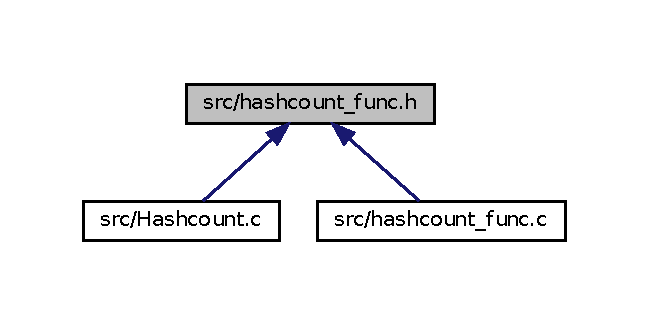
\includegraphics[width=312pt]{hashcount__func_8h__dep__incl}
\end{center}
\end{figure}
\subsection*{Classes}
\begin{DoxyCompactItemize}
\item 
struct \hyperlink{structwordlist}{wordlist}
\begin{DoxyCompactList}\small\item\em Is a header that provides multible Functions for hashlists and wordlists. Author\+: Parzer Florian. \end{DoxyCompactList}\item 
struct \hyperlink{structhashlist}{hashlist}
\begin{DoxyCompactList}\small\item\em A dynamic list of hash buckets. \end{DoxyCompactList}\end{DoxyCompactItemize}
\subsection*{Typedefs}
\begin{DoxyCompactItemize}
\item 
typedef struct \hyperlink{structwordlist}{wordlist} \hyperlink{hashcount__func_8h_a6b5561259b92a62f4c88a80208ea0389}{wordlist}
\begin{DoxyCompactList}\small\item\em Is a header that provides multible Functions for hashlists and wordlists. Author\+: Parzer Florian. \end{DoxyCompactList}\item 
typedef struct \hyperlink{structhashlist}{hashlist} \hyperlink{hashcount__func_8h_a8028004e48db88fd9892da1b97d4bfea}{hashlist}
\begin{DoxyCompactList}\small\item\em A dynamic list of hash buckets. \end{DoxyCompactList}\end{DoxyCompactItemize}
\subsection*{Functions}
\begin{DoxyCompactItemize}
\item 
void \hyperlink{hashcount__func_8h_ad1b217640d5373185b0ab4611b271a86}{read\+File} (\hyperlink{structhashlist}{hashlist} $\ast$$\ast$list, F\+I\+LE $\ast$file)
\begin{DoxyCompactList}\small\item\em Reads the File and fills the hashlist with the words of the file. \end{DoxyCompactList}\item 
void \hyperlink{hashcount__func_8h_ae43c72ed201283355c76a36c3dc99032}{add\+Wordto\+Bucket} (\hyperlink{structhashlist}{hashlist} $\ast$$\ast$list, int hash, char $\ast$word)
\item 
void \hyperlink{hashcount__func_8h_af5ab016cf90d6b793db2d24ab7fe6c0e}{add\+Word} (\hyperlink{structwordlist}{wordlist} $\ast$$\ast$list, char $\ast$word)
\begin{DoxyCompactList}\small\item\em Adds a word to the wordlist. \end{DoxyCompactList}\item 
void \hyperlink{hashcount__func_8h_af406ea8dc323ec35fd3512b182f08999}{free\+Hashlist} (\hyperlink{structhashlist}{hashlist} $\ast$list)
\begin{DoxyCompactList}\small\item\em Frees the with malloc allocated memory of a hashlist. \end{DoxyCompactList}\item 
int \hyperlink{hashcount__func_8h_a02e6d7eb6a614e0f0a00a7cf82805774}{get\+Hash} (char $\ast$word)
\begin{DoxyCompactList}\small\item\em Calculates the hashvalue of a word. \end{DoxyCompactList}\item 
void \hyperlink{hashcount__func_8h_a7ebd0e2c75c007cfa2a268bfce63c5e5}{print\+Hashlist} (\hyperlink{structhashlist}{hashlist} $\ast$list)
\begin{DoxyCompactList}\small\item\em Prints the hashlist in a readable way. \end{DoxyCompactList}\item 
void \hyperlink{hashcount__func_8h_afb73f9700e2348d754dabfbb3f85cd15}{print\+Hash\+Bucket} (\hyperlink{structhashlist}{hashlist} $\ast$list, long bucket)
\begin{DoxyCompactList}\small\item\em Prints on bucket of the hashlist. \end{DoxyCompactList}\item 
void \hyperlink{hashcount__func_8h_a79a2f0a71b4c8bd1716f9cb8d498d766}{print\+Buckets\+Words} (\hyperlink{structwordlist}{wordlist} $\ast$buckets, F\+I\+LE $\ast$file, F\+I\+LE $\ast$output)
\begin{DoxyCompactList}\small\item\em Only the words who have the same hash value as the stated buckets. \end{DoxyCompactList}\item 
void \hyperlink{hashcount__func_8h_a05d5a48c4befa15d197f866d8f8836a5}{print\+Censor\+Buckets} (\hyperlink{structwordlist}{wordlist} $\ast$buckets, F\+I\+LE $\ast$file, F\+I\+LE $\ast$output)
\begin{DoxyCompactList}\small\item\em Prints the text of the input file in the output file and censors the words in the stated buckets. \end{DoxyCompactList}\item 
int \hyperlink{hashcount__func_8h_a8cd45d120ec7408ca1613f1116bf5267}{contains} (char $\ast$word, \hyperlink{structwordlist}{wordlist} $\ast$buchets)
\begin{DoxyCompactList}\small\item\em Checks if the word has the same hash value as one of the buckets. \end{DoxyCompactList}\item 
int \hyperlink{hashcount__func_8h_ad5f58fc748f687d2f75e94502d8626c6}{compare\+Wordlist} (\hyperlink{structwordlist}{wordlist} $\ast$list1, \hyperlink{structwordlist}{wordlist} $\ast$list2)
\end{DoxyCompactItemize}


\subsection{Typedef Documentation}
\mbox{\Hypertarget{hashcount__func_8h_a8028004e48db88fd9892da1b97d4bfea}\label{hashcount__func_8h_a8028004e48db88fd9892da1b97d4bfea}} 
\index{hashcount\+\_\+func.\+h@{hashcount\+\_\+func.\+h}!hashlist@{hashlist}}
\index{hashlist@{hashlist}!hashcount\+\_\+func.\+h@{hashcount\+\_\+func.\+h}}
\subsubsection{\texorpdfstring{hashlist}{hashlist}}
{\footnotesize\ttfamily typedef struct \hyperlink{structhashlist}{hashlist} \hyperlink{structhashlist}{hashlist}}



A dynamic list of hash buckets. 

It is a dynamic list where each element has a pointer to the next element, a pointer to a wordlist and the hash value \mbox{\Hypertarget{hashcount__func_8h_a6b5561259b92a62f4c88a80208ea0389}\label{hashcount__func_8h_a6b5561259b92a62f4c88a80208ea0389}} 
\index{hashcount\+\_\+func.\+h@{hashcount\+\_\+func.\+h}!wordlist@{wordlist}}
\index{wordlist@{wordlist}!hashcount\+\_\+func.\+h@{hashcount\+\_\+func.\+h}}
\subsubsection{\texorpdfstring{wordlist}{wordlist}}
{\footnotesize\ttfamily typedef struct \hyperlink{structwordlist}{wordlist} \hyperlink{structwordlist}{wordlist}}



Is a header that provides multible Functions for hashlists and wordlists. Author\+: Parzer Florian. 

A dynamic list of words

It is a dynamic list where eac element has a pointer to the next element, an integer variable that is used for counting and the word itself 

\subsection{Function Documentation}
\mbox{\Hypertarget{hashcount__func_8h_af5ab016cf90d6b793db2d24ab7fe6c0e}\label{hashcount__func_8h_af5ab016cf90d6b793db2d24ab7fe6c0e}} 
\index{hashcount\+\_\+func.\+h@{hashcount\+\_\+func.\+h}!add\+Word@{add\+Word}}
\index{add\+Word@{add\+Word}!hashcount\+\_\+func.\+h@{hashcount\+\_\+func.\+h}}
\subsubsection{\texorpdfstring{add\+Word()}{addWord()}}
{\footnotesize\ttfamily void add\+Word (\begin{DoxyParamCaption}\item[{\hyperlink{structwordlist}{wordlist} $\ast$$\ast$}]{list,  }\item[{char $\ast$}]{word }\end{DoxyParamCaption})}



Adds a word to the wordlist. 

Adds the word to the wordlist. If the word is already contained a counter is increased.


\begin{DoxyParams}{Parameters}
{\em list} & Is the wordlist in which the word is added. If it is N\+U\+LL, the list will be created. \\
\hline
{\em word} & The word the hash is calculated from. \\
\hline
\end{DoxyParams}
\mbox{\Hypertarget{hashcount__func_8h_ae43c72ed201283355c76a36c3dc99032}\label{hashcount__func_8h_ae43c72ed201283355c76a36c3dc99032}} 
\index{hashcount\+\_\+func.\+h@{hashcount\+\_\+func.\+h}!add\+Wordto\+Bucket@{add\+Wordto\+Bucket}}
\index{add\+Wordto\+Bucket@{add\+Wordto\+Bucket}!hashcount\+\_\+func.\+h@{hashcount\+\_\+func.\+h}}
\subsubsection{\texorpdfstring{add\+Wordto\+Bucket()}{addWordtoBucket()}}
{\footnotesize\ttfamily void add\+Wordto\+Bucket (\begin{DoxyParamCaption}\item[{\hyperlink{structhashlist}{hashlist} $\ast$$\ast$}]{list,  }\item[{int}]{hash,  }\item[{char $\ast$}]{word }\end{DoxyParamCaption})}

\mbox{\Hypertarget{hashcount__func_8h_ad5f58fc748f687d2f75e94502d8626c6}\label{hashcount__func_8h_ad5f58fc748f687d2f75e94502d8626c6}} 
\index{hashcount\+\_\+func.\+h@{hashcount\+\_\+func.\+h}!compare\+Wordlist@{compare\+Wordlist}}
\index{compare\+Wordlist@{compare\+Wordlist}!hashcount\+\_\+func.\+h@{hashcount\+\_\+func.\+h}}
\subsubsection{\texorpdfstring{compare\+Wordlist()}{compareWordlist()}}
{\footnotesize\ttfamily int compare\+Wordlist (\begin{DoxyParamCaption}\item[{\hyperlink{structwordlist}{wordlist} $\ast$}]{list1,  }\item[{\hyperlink{structwordlist}{wordlist} $\ast$}]{list2 }\end{DoxyParamCaption})}

\mbox{\Hypertarget{hashcount__func_8h_a8cd45d120ec7408ca1613f1116bf5267}\label{hashcount__func_8h_a8cd45d120ec7408ca1613f1116bf5267}} 
\index{hashcount\+\_\+func.\+h@{hashcount\+\_\+func.\+h}!contains@{contains}}
\index{contains@{contains}!hashcount\+\_\+func.\+h@{hashcount\+\_\+func.\+h}}
\subsubsection{\texorpdfstring{contains()}{contains()}}
{\footnotesize\ttfamily int contains (\begin{DoxyParamCaption}\item[{char $\ast$}]{word,  }\item[{\hyperlink{structwordlist}{wordlist} $\ast$}]{buckets }\end{DoxyParamCaption})}



Checks if the word has the same hash value as one of the buckets. 

Checks if the word has the same hash value as one of the buckets by comparing it to every element of the wordlist.


\begin{DoxyParams}{Parameters}
{\em word} & Is the word that is checked \\
\hline
{\em buckets} & Are the hash values that are compaired against \\
\hline
\end{DoxyParams}
\begin{DoxyReturn}{Returns}
1 if the word has the same hashv alue as one of the buckets, otherwise it will return 0 
\end{DoxyReturn}
\mbox{\Hypertarget{hashcount__func_8h_af406ea8dc323ec35fd3512b182f08999}\label{hashcount__func_8h_af406ea8dc323ec35fd3512b182f08999}} 
\index{hashcount\+\_\+func.\+h@{hashcount\+\_\+func.\+h}!free\+Hashlist@{free\+Hashlist}}
\index{free\+Hashlist@{free\+Hashlist}!hashcount\+\_\+func.\+h@{hashcount\+\_\+func.\+h}}
\subsubsection{\texorpdfstring{free\+Hashlist()}{freeHashlist()}}
{\footnotesize\ttfamily void free\+Hashlist (\begin{DoxyParamCaption}\item[{\hyperlink{structhashlist}{hashlist} $\ast$}]{list }\end{DoxyParamCaption})}



Frees the with malloc allocated memory of a hashlist. 

It iterates over every element of the hashlist and frees every element that reserved its memory with the melloc method


\begin{DoxyParams}{Parameters}
{\em list} & The hashlist that schould be freed \\
\hline
\end{DoxyParams}
\mbox{\Hypertarget{hashcount__func_8h_a02e6d7eb6a614e0f0a00a7cf82805774}\label{hashcount__func_8h_a02e6d7eb6a614e0f0a00a7cf82805774}} 
\index{hashcount\+\_\+func.\+h@{hashcount\+\_\+func.\+h}!get\+Hash@{get\+Hash}}
\index{get\+Hash@{get\+Hash}!hashcount\+\_\+func.\+h@{hashcount\+\_\+func.\+h}}
\subsubsection{\texorpdfstring{get\+Hash()}{getHash()}}
{\footnotesize\ttfamily int get\+Hash (\begin{DoxyParamCaption}\item[{char $\ast$}]{word }\end{DoxyParamCaption})}



Calculates the hashvalue of a word. 

Calculates the bash of the word by summing the values of the characters and calculate the result withc modulo


\begin{DoxyParams}{Parameters}
{\em word} & The word the hash is calculated from\\
\hline
\end{DoxyParams}
\begin{DoxyReturn}{Returns}
returns the calculated hashvalue as Integer 
\end{DoxyReturn}
\mbox{\Hypertarget{hashcount__func_8h_a79a2f0a71b4c8bd1716f9cb8d498d766}\label{hashcount__func_8h_a79a2f0a71b4c8bd1716f9cb8d498d766}} 
\index{hashcount\+\_\+func.\+h@{hashcount\+\_\+func.\+h}!print\+Buckets\+Words@{print\+Buckets\+Words}}
\index{print\+Buckets\+Words@{print\+Buckets\+Words}!hashcount\+\_\+func.\+h@{hashcount\+\_\+func.\+h}}
\subsubsection{\texorpdfstring{print\+Buckets\+Words()}{printBucketsWords()}}
{\footnotesize\ttfamily void print\+Buckets\+Words (\begin{DoxyParamCaption}\item[{\hyperlink{structwordlist}{wordlist} $\ast$}]{buckets,  }\item[{F\+I\+LE $\ast$}]{file,  }\item[{F\+I\+LE $\ast$}]{output }\end{DoxyParamCaption})}



Only the words who have the same hash value as the stated buckets. 

It prints only the words that\textquotesingle{}s hash maches one of the buckets. Every other character of the input file will not be printed.


\begin{DoxyParams}{Parameters}
{\em buckets} & The hash values of the stated buckets \\
\hline
{\em file} & The input file stream \\
\hline
{\em output} & The output file stream \\
\hline
\end{DoxyParams}
\mbox{\Hypertarget{hashcount__func_8h_a05d5a48c4befa15d197f866d8f8836a5}\label{hashcount__func_8h_a05d5a48c4befa15d197f866d8f8836a5}} 
\index{hashcount\+\_\+func.\+h@{hashcount\+\_\+func.\+h}!print\+Censor\+Buckets@{print\+Censor\+Buckets}}
\index{print\+Censor\+Buckets@{print\+Censor\+Buckets}!hashcount\+\_\+func.\+h@{hashcount\+\_\+func.\+h}}
\subsubsection{\texorpdfstring{print\+Censor\+Buckets()}{printCensorBuckets()}}
{\footnotesize\ttfamily void print\+Censor\+Buckets (\begin{DoxyParamCaption}\item[{\hyperlink{structwordlist}{wordlist} $\ast$}]{buckets,  }\item[{F\+I\+LE $\ast$}]{file,  }\item[{F\+I\+LE $\ast$}]{output }\end{DoxyParamCaption})}



Prints the text of the input file in the output file and censors the words in the stated buckets. 

It prints every character of the input file in the output file. If the word is contained in the stated buckets it will be censored.


\begin{DoxyParams}{Parameters}
{\em buckets} & The hash values of the stated buckets \\
\hline
{\em file} & The input file stream \\
\hline
{\em output} & The output file stream \\
\hline
\end{DoxyParams}
\mbox{\Hypertarget{hashcount__func_8h_afb73f9700e2348d754dabfbb3f85cd15}\label{hashcount__func_8h_afb73f9700e2348d754dabfbb3f85cd15}} 
\index{hashcount\+\_\+func.\+h@{hashcount\+\_\+func.\+h}!print\+Hash\+Bucket@{print\+Hash\+Bucket}}
\index{print\+Hash\+Bucket@{print\+Hash\+Bucket}!hashcount\+\_\+func.\+h@{hashcount\+\_\+func.\+h}}
\subsubsection{\texorpdfstring{print\+Hash\+Bucket()}{printHashBucket()}}
{\footnotesize\ttfamily void print\+Hash\+Bucket (\begin{DoxyParamCaption}\item[{\hyperlink{structhashlist}{hashlist} $\ast$}]{list,  }\item[{long}]{bucket }\end{DoxyParamCaption})}



Prints on bucket of the hashlist. 

Prints the stated bucket. If the words per line exeed 10 a new line is started. If the Bucket is not found it will print an error Message.


\begin{DoxyParams}{Parameters}
{\em list} & The hashlist in which the bucket will be searched in. \\
\hline
{\em bucket} & The hashvalue of the bucket that should be printed. \\
\hline
\end{DoxyParams}
\mbox{\Hypertarget{hashcount__func_8h_a7ebd0e2c75c007cfa2a268bfce63c5e5}\label{hashcount__func_8h_a7ebd0e2c75c007cfa2a268bfce63c5e5}} 
\index{hashcount\+\_\+func.\+h@{hashcount\+\_\+func.\+h}!print\+Hashlist@{print\+Hashlist}}
\index{print\+Hashlist@{print\+Hashlist}!hashcount\+\_\+func.\+h@{hashcount\+\_\+func.\+h}}
\subsubsection{\texorpdfstring{print\+Hashlist()}{printHashlist()}}
{\footnotesize\ttfamily void print\+Hashlist (\begin{DoxyParamCaption}\item[{\hyperlink{structhashlist}{hashlist} $\ast$}]{list }\end{DoxyParamCaption})}



Prints the hashlist in a readable way. 

Prints every bucket of the Hashlist in a seperate line. If the words per line exeed 10 a new line is started


\begin{DoxyParams}{Parameters}
{\em list} & The hashlist that will be printed. \\
\hline
\end{DoxyParams}
\mbox{\Hypertarget{hashcount__func_8h_ad1b217640d5373185b0ab4611b271a86}\label{hashcount__func_8h_ad1b217640d5373185b0ab4611b271a86}} 
\index{hashcount\+\_\+func.\+h@{hashcount\+\_\+func.\+h}!read\+File@{read\+File}}
\index{read\+File@{read\+File}!hashcount\+\_\+func.\+h@{hashcount\+\_\+func.\+h}}
\subsubsection{\texorpdfstring{read\+File()}{readFile()}}
{\footnotesize\ttfamily void read\+File (\begin{DoxyParamCaption}\item[{\hyperlink{structhashlist}{hashlist} $\ast$$\ast$}]{list,  }\item[{F\+I\+LE $\ast$}]{file }\end{DoxyParamCaption})}



Reads the File and fills the hashlist with the words of the file. 

The method reads the file. It splits the stream at the charackters \textquotesingle{}newline\textquotesingle{}, \textquotesingle{}space\textquotesingle{}, \textquotesingle{}.\textquotesingle{}, \textquotesingle{}\+:\textquotesingle{}, \textquotesingle{},\textquotesingle{}, \textquotesingle{};\textquotesingle{}, \textquotesingle{}?\textquotesingle{} and \textquotesingle{}space\textquotesingle{}. Afterwards it stores the words in the hashlist


\begin{DoxyParams}{Parameters}
{\em list} & The hashlist to which the word is added. \\
\hline
{\em file} & The File Stream of the Input file \\
\hline
\end{DoxyParams}

%--- End generated contents ---

% Index
\backmatter
\newpage
\phantomsection
\clearemptydoublepage
\addcontentsline{toc}{chapter}{Index}
\printindex

\end{document}
